\formulasheettitle{Transformer Model}%
  {Formula sheet for a three-phase two-winding transformer}
	\begin{noteBox}
		\textbf{Notation.} Indices $k=1,2,3$ identify the transformer legs or phases;
		$p$ and $s$ denote the primary and secondary windings. Uppercase $U$ and $I$
		denote electrical quantities, $\Phi$ the magnetic flux, $\Psi=N\Phi$ the flux
		linkage, and $\Theta=NI$ the magnetomotive force. The example uses vector group
		$\mathrm{Yy0}$.
	\end{noteBox}
	
	\begin{formulaBox}{Transformer-leg equations}
		For each leg $k\in\{1,2,3\}$, the reluctance associated with the iron-loss
		resistance is
		\begin{equation}
			\Rmag_{R\mathrm{Fe}}=\frac{N_1^2}{R_{\mathrm{Fe}}}.
		\end{equation}
		The nonlinear magnetizing characteristic is represented by
		\begin{equation}
			\Theta_{\mu k}=N_1 I_{\mu N}
			\left[
			a\frac{\Phi_k}{\Phi_N}
			+(1-a)\left(\frac{\Phi_k}{\Phi_N}\right)^m
			\right],
			\qquad k=1,2,3.
		\end{equation}
		Equivalently, the magnetizing current of one leg is
		\begin{equation}
			I_{\mu k}=I_{\mu N}
			\left[
			a\frac{\Phi_k}{\Phi_N}
			+(1-a)\left(\frac{\Phi_k}{\Phi_N}\right)^m
			\right].
		\end{equation}
	\end{formulaBox}
	
	\begin{formulaBox}{Primary-winding equations}
		For every phase $k$,
		\begin{align}
			\Phi_{kp}
			&=\frac{\Psi_{kp}}{N_1}
			=\frac{1}{N_1}\int\!\left(U_{kp}-R_1I_{kp}\right)\diff t,
			& I_{kp}&=\frac{\Theta_k}{N_1}.
		\end{align}
		Written separately for the three phases, this relation applies for
		$k=1$, $2$, and $3$ with the corresponding phase quantities.
	\end{formulaBox}
	
	\begin{formulaBox}{Secondary-winding equations}
		For every phase $k$,
		\begin{align}
			\Phi_{ks}
			&=\frac{\Psi_{ks}}{N_2}
			=\frac{1}{N_2}\int\!\left(U_{ks}-R_2I_{ks}\right)\diff t,
			& I_{ks}&=\frac{\Theta_k}{N_2}.
		\end{align}
		The voltage and current reference directions must be chosen consistently with
		the winding polarities used in the circuit model.
	\end{formulaBox}
	
	\newpage
	\thispagestyle{scrheadings}
	
	\begin{formulaBox}{Common core flux and winding flux linkages}
		For ideal magnetic coupling of the windings on each leg,
		\begin{equation}
			\Phi_{kp}=\Phi_{ks}=\Phi_k,
			\qquad k=1,2,3.
		\end{equation}
		The corresponding flux linkages are
		\begin{equation}
			\Psi_{kp}=N_1\Phi_k,
			\qquad
			\Psi_{ks}=N_2\Phi_k.
		\end{equation}
		Thus, in general,
		\begin{equation}
			\Psi_{kp}\ne\Psi_{ks}\quad\text{when}\quad N_1\ne N_2,
		\end{equation}
		even though both windings link the same core flux $\Phi_k$.
	\end{formulaBox}
	
	\begin{formulaBox}{Leakage-flux branch}
		With $\Rmag_{\Phi\sigma}$ denoting the equivalent magnetic reluctance of the
		leakage path,
		\begin{equation}
			\Phi_{k\sigma}=\frac{\Theta_k}{\Rmag_{\Phi\sigma}},
			\qquad k=1,2,3.
		\end{equation}
		For a leakage inductance $L_{1\sigma}$ referred to the primary winding,
		\begin{equation}
			L_{1\sigma}=\frac{N_1^2}{\Rmag_{\Phi\sigma}}
			\qquad\Longleftrightarrow\qquad
			\Rmag_{\Phi\sigma}=\frac{N_1^2}{L_{1\sigma}}.
		\end{equation}
	\end{formulaBox}
	
	\begin{formulaBox}{Tank representation}
		The tank is represented by an additional magnetic reluctance $\Rmag_{\mathrm{tank}}$.
		The source text recommends the following approximate choices:
		\begin{align}
			\Rmag_{\mathrm{tank}}
			&\approx (0.1\ldots0.01)\frac{N_1^2}{L_{1\sigma}},
			&&\text{rough initial estimate: 10–100 times the leakage inductance},\\
			\Rmag_{\mathrm{tank}}
			&\approx 10^5\ldots10^6,
			&&\text{tank magnetic reluctance in the model units},\\
			\Rmag_{\mathrm{tank}}
			&\approx 10^{20},
			&&\text{tank branch absent (practically open)}.
		\end{align}
	\end{formulaBox}
	
	
	\newpage
	\thispagestyle{scrheadings}
	
%	\begin{formulaBox}{Rated data: 300 MVA, 400 kV / 120 kV, 50 Hz}
%		\renewcommand{\arraystretch}{\formulaTableStretch}
%		\begin{tabularx}{\textwidth}{>{\bfseries\(}l<{\)} >{\(}l<{\)} X}
%			\toprule
%			\text{Symbol} & \text{Value} & \textbf{Meaning} \\
%			\midrule
%			S_N & 300\times10^6\ \mathrm{VA} & Three-phase rated apparent power \\
%			U_{1N,LL} & 400\times10^3\ \mathrm{V} & Primary rated line-to-line voltage \\
%			U_{2N,LL} & 120\times10^3\ \mathrm{V} & Secondary rated line-to-line voltage \\
%			f_N & 50\ \mathrm{Hz} & Rated frequency \\
%			N_1 & 1000 & Primary number of turns \\
%			u_R & 0.002 & Resistive part of relative short-circuit voltage \\
%			u_X & 0.2 & Inductive part of relative short-circuit voltage \\
%			i_0 & 0.0006 & Relative no-load current \\
%			p_0 & 0.0004 & Relative no-load loss, with $p_0<i_0$ \\
%			a & 0.75 & Linear weighting in the magnetizing characteristic \\
%			m & 9 & Exponent of the nonlinear magnetizing term \\
%			\bottomrule
%		\end{tabularx}
%	\end{formulaBox}

	\begin{formulaBox}{Transformer main data:}
			\renewcommand{\arraystretch}{\formulaTableStretch}
			\begin{tabularx}{\textwidth}{>{\bfseries\(}l<{\)} >{\text{}}l X}
					\toprule
					\text{Symbol} & \textbf{Meaning} \\
					\midrule
					S_N & Three-phase rated apparent power \\
					U_{1N,LL} & Primary rated line-to-line voltage \\
					U_{2N,LL} & Secondary rated line-to-line voltage \\
					f_N & Rated frequency \\
					N_1 & Primary number of turns \\
					u_R & Resistive part of relative short-circuit voltage \\
					u_X & Inductive part of relative short-circuit voltage \\
					i_0 & Relative no-load current \\
					p_0 & Relative no-load loss, with $p_0<i_0$ \\
					a & Linear weighting in the magnetizing characteristic \\
					m & Exponent of the nonlinear magnetizing term \\
					\bottomrule
			\end{tabularx}
	\end{formulaBox}
	
	\begin{formulaBox}{Per-leg quantities for vector group $\mathrm{Yy0}$}
		The three-phase values are first converted to one transformer leg:
		\begin{align}
			S_{N,\mathrm{leg}} &= \frac{S_N}{3}, &
			U_{1N} &= \frac{U_{1N,LL}}{\sqrt{3}}, &
			U_{2N} &= \frac{U_{2N,LL}}{\sqrt{3}},\\
			I_{1N} &= \frac{S_{N,\mathrm{leg}}}{U_{1N}}, &
			Z_{1N} &= \frac{U_{1N}}{I_{1N}}, &
			\omega_N &= 2\pi f_N.
		\end{align}
	\end{formulaBox}
	
	\begin{formulaBox}{Winding and iron-loss parameters}
		The short-circuit impedance is split equally between the two windings and
		referred initially to the primary side:
		\begin{align}
			R_1 &= \frac{Z_{1N}u_R}{2}, &
			L_{1\sigma} &= \frac{Z_{1N}u_X}{2\omega_N},\\
			R_{\mathrm{Fe}} &= \frac{U_{1N}^2}{p_0S_{N,\mathrm{leg}}}, &
			\Rmag_{R\mathrm{Fe}} &= \frac{N_1^2}{R_{\mathrm{Fe}}},\\
			N_2 &= N_1\frac{U_{2N}}{U_{1N}}, &
			R_2 &= R_1\left(\frac{N_2}{N_1}\right)^2,\\
			\Rmag_{\Phi\sigma} &= \frac{N_1^2}{L_{1\sigma}}. &&
		\end{align}
	\end{formulaBox}
	
	\newpage
	\thispagestyle{scrheadings}
	
	\begin{formulaBox}{Magnetizing branch and rated flux}
		From the no-load current and no-load losses,
		\begin{align}
			X_h &= \frac{U_{1N}^2}
			{S_{N,\mathrm{leg}}\sqrt{i_0^2-p_0^2}},\\
			I_\mu &= \frac{U_{1N}}{X_h},\\
			I_{\mu N} &= \sqrt{2}\,I_\mu,\\
			\Phi_N &= \frac{\sqrt{2}\,U_{1N}}{\omega_NN_1}.
		\end{align}
		The nonlinear characteristic then becomes
		\begin{equation}
			I_\mu(\Phi)=I_{\mu N}
			\left[
			a\frac{\Phi}{\Phi_N}
			+(1-a)\left(\frac{\Phi}{\Phi_N}\right)^m
			\right].
		\end{equation}
	\end{formulaBox}
	
	\begin{formulaBox}{Parameter definitions}
		\renewcommand{\arraystretch}{\formulaTableStretch}
		\begin{tabularx}{\textwidth}{>{\bfseries\(}l<{\)} X}
			\toprule
			\text{Symbol} & \textbf{Meaning} \\
			\midrule
			\Theta_k & Magnetomotive force of leg $k$ \\
			\Phi_k,\ \Phi_{k\sigma} & Main and leakage fluxes of leg $k$ \\
			\Psi_{kp},\ \Psi_{ks} & Primary and secondary flux linkages \\
			\Rmag_{R\mathrm{Fe}} & Magnetic reluctance associated with the iron-loss branch \\
			\Rmag_{\Phi\sigma} & Equivalent leakage-path reluctance \\
			\Rmag_{\mathrm{tank}} & Tank-path magnetic reluctance \\
			R_1,\ R_2 & Primary and secondary winding resistances \\
			R_{\mathrm{Fe}} & Equivalent iron-loss resistance \\
			L_{1\sigma} & Primary-referred leakage inductance \\
			X_h & Main magnetizing reactance \\
			I_{\mu N},\ \Phi_N & Rated peak magnetizing current and rated peak flux \\
			a,\ m & Shape parameters of the nonlinear magnetization curve \\
			\bottomrule
		\end{tabularx}
	\end{formulaBox}
	
	\begin{noteBox}
		\textbf{Implementation notes.} The time integrals may be implemented with
		behavioural sources in LTspice. When forming the winding equations, verify the
		chosen voltage polarities, current reference directions, initial flux, and the
		sign of each magnetomotive-force contribution. The numerical tank-reluctance
		range is model- and unit-dependent and should be validated against the intended
		zero-sequence behaviour.
	\end{noteBox}
	
	\vfill
%	{\small\color{muted}\sffamily
%		Typeset from the supplied transformer-model notes. English wording and notation
%		have been standardized; explicitly identified dimensional inconsistencies in
%		the source have been corrected.}

	\begin{formulaBox}{Rated data: 300 MVA, 400 kV / 120 kV, 50 Hz}
			\renewcommand{\arraystretch}{\formulaTableStretch}
			\begin{tabularx}{\textwidth}{>{\bfseries\(}l<{\)} >{\(}l<{\)} X}
					\toprule
					\text{Symbol} & \text{Value} & \textbf{Meaning} \\
					\midrule
					S_N & 300\times10^6\ \mathrm{VA} & Three-phase rated apparent power \\
					U_{1N,LL} & 400\times10^3\ \mathrm{V} & Primary rated line-to-line voltage \\
					U_{2N,LL} & 120\times10^3\ \mathrm{V} & Secondary rated line-to-line voltage \\
					f_N & 50\ \mathrm{Hz} & Rated frequency \\
					N_1 & 1000 & Primary number of turns \\
					u_R & 0.002 & Resistive part of relative short-circuit voltage \\
					u_X & 0.2 & Inductive part of relative short-circuit voltage \\
					i_0 & 0.0006 & Relative no-load current \\
					p_0 & 0.0004 & Relative no-load loss, with $p_0<i_0$ \\
					a & 0.75 & Linear weighting in the magnetizing characteristic \\
					m & 9 & Exponent of the nonlinear magnetizing term \\
					\bottomrule
			\end{tabularx}
	\end{formulaBox}
	
% LaTeX fragment for direct insertion into a book chapter.
% Required definitions/packages are provided by the central preamble:
% formulaBox, noteBox, amsmath, booktabs, tabularx, siunitx.

\begin{noteBox}
	\textbf{Assumptions.}
	The calculation uses a balanced per-phase equivalent circuit for vector group
	$\mathrm{Yy0}$. The total short-circuit resistance and leakage reactance are
	split equally between the primary winding and the secondary winding referred
	to the primary side. All magnetizing-branch quantities are initially referred
	to the \SI{400}{\kilo\volt} side.
\end{noteBox}

\begin{formulaBox}{Per-leg rated quantities}
	The three-phase rated values are converted to one transformer leg:
	\begin{align}
		S_{N,\mathrm{leg}}
		&=\frac{S_N}{3}
		=\frac{\SI{300}{\mega\volt\ampere}}{3}
		=\SI{100}{\mega\volt\ampere},\\
		U_{1N}
		&=\frac{U_{1N,LL}}{\sqrt{3}}
		=\frac{\SI{400}{\kilo\volt}}{\sqrt{3}}
		=\SI{230.940}{\kilo\volt},\\
		U_{2N}
		&=\frac{U_{2N,LL}}{\sqrt{3}}
		=\frac{\SI{120}{\kilo\volt}}{\sqrt{3}}
		=\SI{69.282}{\kilo\volt},\\
		I_{1N}
		&=\frac{S_{N,\mathrm{leg}}}{U_{1N}}
		=\SI{433.013}{\ampere},\\
		Z_{1N}
		&=\frac{U_{1N}}{I_{1N}}
		=\frac{U_{1N,LL}^{2}}{S_N}
		=\SI{533.333}{\ohm},\\
		\omega_N
		&=2\pi f_N
		=\SI{314.159}{\radian\per\second}.
	\end{align}
	
	The turns ratio and secondary number of turns are
	\begin{align}
		u=\frac{N_1}{N_2}
		&=\frac{U_{1N}}{U_{2N}}
		=\frac{400}{120}
		=3.33333,\\
		N_2&=N_1\frac{U_{2N}}{U_{1N}}
		=1000\frac{120}{400}
		=\boxed{300}.
	\end{align}
\end{formulaBox}

\begin{formulaBox}{Winding parameters}
	The total short-circuit resistance and leakage reactance referred to the
	primary side are
	\begin{align}
		R_k'&=u_R Z_{1N}
		=0.002\cdot\SI{533.333}{\ohm}
		=\SI{1.06667}{\ohm},\\
		X_{k\sigma}'&=u_X Z_{1N}
		=0.2\cdot\SI{533.333}{\ohm}
		=\SI{106.667}{\ohm},\\
		L_{k\sigma}'&=\frac{X_{k\sigma}'}{\omega_N}
		=\SI{0.339531}{\henry}.
	\end{align}
	
	With equal division between the two windings,
	\begin{align}
		R_1=R_2'
		&=\frac{R_k'}{2}
		=\boxed{\SI{0.533333}{\ohm}},\\
		L_{1\sigma}=L_{2\sigma}'
		&=\frac{L_{k\sigma}'}{2}
		=\boxed{\SI{0.169765}{\henry}}.
	\end{align}
	
	The actual secondary-side parameters follow from
	$(N_2/N_1)^2=0.09$:
	\begin{align}
		R_2&=R_2'\left(\frac{N_2}{N_1}\right)^2
		=\SI{0.533333}{\ohm}\cdot0.09
		=\boxed{\SI{0.048000}{\ohm}},\\
		L_{2\sigma}&=L_{2\sigma}'\left(\frac{N_2}{N_1}\right)^2
		=\SI{0.169765}{\henry}\cdot0.09
		=\boxed{\SI{0.0152789}{\henry}}.
	\end{align}
	
	For the magnetic-circuit leakage representation,
	\begin{equation}
		\Rmag_{\Phi\sigma}
		=\frac{N_1^2}{L_{1\sigma}}
		=\frac{1000^2}{\SI{0.169765}{\henry}}
		=\boxed{\SI{5.89049e6}{\per\henry}}.
	\end{equation}
\end{formulaBox}

\begin{formulaBox}{Iron-loss parameters}
	The total rated no-load loss is
	\begin{equation}
		P_0=p_0S_N
		=0.0004\cdot\SI{300}{\mega\volt\ampere}
		=\SI{120}{\kilo\watt}.
	\end{equation}
	
	Thus, each transformer leg represents
	\SI{40}{\kilo\watt} of iron loss. The primary-referred iron-loss resistance is
	\begin{align}
		R_{\mathrm{Fe}}
		&=\frac{U_{1N}^{2}}{p_0S_{N,\mathrm{leg}}}\\
		&=\frac{(\SI{230.940}{\kilo\volt})^2}
		{0.0004\cdot\SI{100}{\mega\volt\ampere}}
		=\boxed{\SI{1.33333}{\mega\ohm}}.
	\end{align}
	
	The corresponding RMS iron-loss current per phase is
	\begin{equation}
		I_{\mathrm{Fe}}
		=\frac{U_{1N}}{R_{\mathrm{Fe}}}
		=\boxed{\SI{0.173205}{\ampere}}.
	\end{equation}
	
	In the magnetic-circuit representation used by the transformer model,
	\begin{equation}
		\Rmag_{R\mathrm{Fe}}
		=\frac{N_1^2}{R_{\mathrm{Fe}}}
		=\frac{1000^2}{\SI{1.33333e6}{\ohm}}
		=\boxed{0.750000}.
	\end{equation}
\end{formulaBox}

\begin{formulaBox}{Magnetizing branch and rated flux}
	The rated RMS no-load current is
	\begin{equation}
		I_0=i_0I_{1N}
		=0.0006\cdot\SI{433.013}{\ampere}
		=\SI{0.259808}{\ampere}.
	\end{equation}
	
	After subtracting the active iron-loss component vectorially, the RMS
	magnetizing current is
	\begin{align}
		I_\mu
		&=I_{1N}\sqrt{i_0^2-p_0^2}\\
		&=\SI{433.013}{\ampere}
		\sqrt{0.0006^2-0.0004^2}
		=\boxed{\SI{0.193649}{\ampere}}.
	\end{align}
	
	The magnetizing reactance and inductance referred to the primary side are
	\begin{align}
		X_h
		&=\frac{U_{1N}}{I_\mu}
		=\frac{U_{1N}^2}
		{S_{N,\mathrm{leg}}\sqrt{i_0^2-p_0^2}}
		=\boxed{\SI{1.19257}{\mega\ohm}},\\
		L_h
		&=\frac{X_h}{\omega_N}
		=\boxed{\SI{3.79607e3}{\henry}}.
	\end{align}
	
	The peak magnetizing current used in the nonlinear characteristic is
	\begin{equation}
		I_{\mu N}=\sqrt{2}\,I_\mu
		=\boxed{\SI{0.273861}{\ampere}}.
	\end{equation}
	
	For a sinusoidal phase voltage, the rated peak core flux is
	\begin{align}
		\Phi_N
		&=\frac{\sqrt{2}\,U_{1N}}{\omega_NN_1}\\
		&=\frac{\sqrt{2}\cdot\SI{230.940}{\kilo\volt}}
		{\SI{314.159}{\radian\per\second}\cdot1000}
		=\boxed{\SI{1.03960}{\weber}}.
	\end{align}
	
	With $a=0.75$ and $m=9$, the numerical magnetizing characteristic becomes
	\begin{equation}
		I_\mu(\Phi)
		=\SI{0.273861}{\ampere}
		\left[
		0.75\frac{\Phi}{\SI{1.03960}{\weber}}
		+0.25\left(\frac{\Phi}{\SI{1.03960}{\weber}}\right)^9
		\right].
	\end{equation}
\end{formulaBox}

\begin{formulaBox}{Calculated parameter summary}
	\renewcommand{\arraystretch}{\formulaTableStretch}
	\begin{tabularx}{\textwidth}{>{\bfseries\(}l<{\)} >{\(}l<{\)} X}
		\toprule
		\text{Parameter} & \text{Calculated value} & \textbf{Reference} \\
		\midrule
		N_2 & 300 & Secondary number of turns \\
		R_1 & \SI{0.533333}{\ohm} & Primary winding resistance \\
		L_{1\sigma} & \SI{0.169765}{\henry} & Primary leakage inductance \\
		R_2' & \SI{0.533333}{\ohm} & Secondary resistance referred to primary \\
		L_{2\sigma}' & \SI{0.169765}{\henry} & Secondary leakage inductance referred to primary \\
		R_2 & \SI{0.048000}{\ohm} & Actual secondary resistance \\
		L_{2\sigma} & \SI{0.0152789}{\henry} & Actual secondary leakage inductance \\
		R_{\mathrm{Fe}} & \SI{1.33333}{\mega\ohm} & Iron-loss resistance, primary-referred \\
		X_h & \SI{1.19257}{\mega\ohm} & Magnetizing reactance, primary-referred \\
		L_h & \SI{3.79607e3}{\henry} & Linear magnetizing inductance \\
		I_{\mu N} & \SI{0.273861}{\ampere} & Rated peak magnetizing current \\
		\Phi_N & \SI{1.03960}{\weber} & Rated peak core flux \\
		\Rmag_{R\mathrm{Fe}} & 0.750000 & Iron-loss magnetic-model parameter \\
		\Rmag_{\Phi\sigma} & \SI{5.89049e6}{\per\henry} & Leakage-path magnetic parameter \\
		\bottomrule
	\end{tabularx}
\end{formulaBox}


\begin{widefigure}{Electrical and magnetic model of a three-phase Yy0 transformer with a three-leg core}{fig:schematic1}
	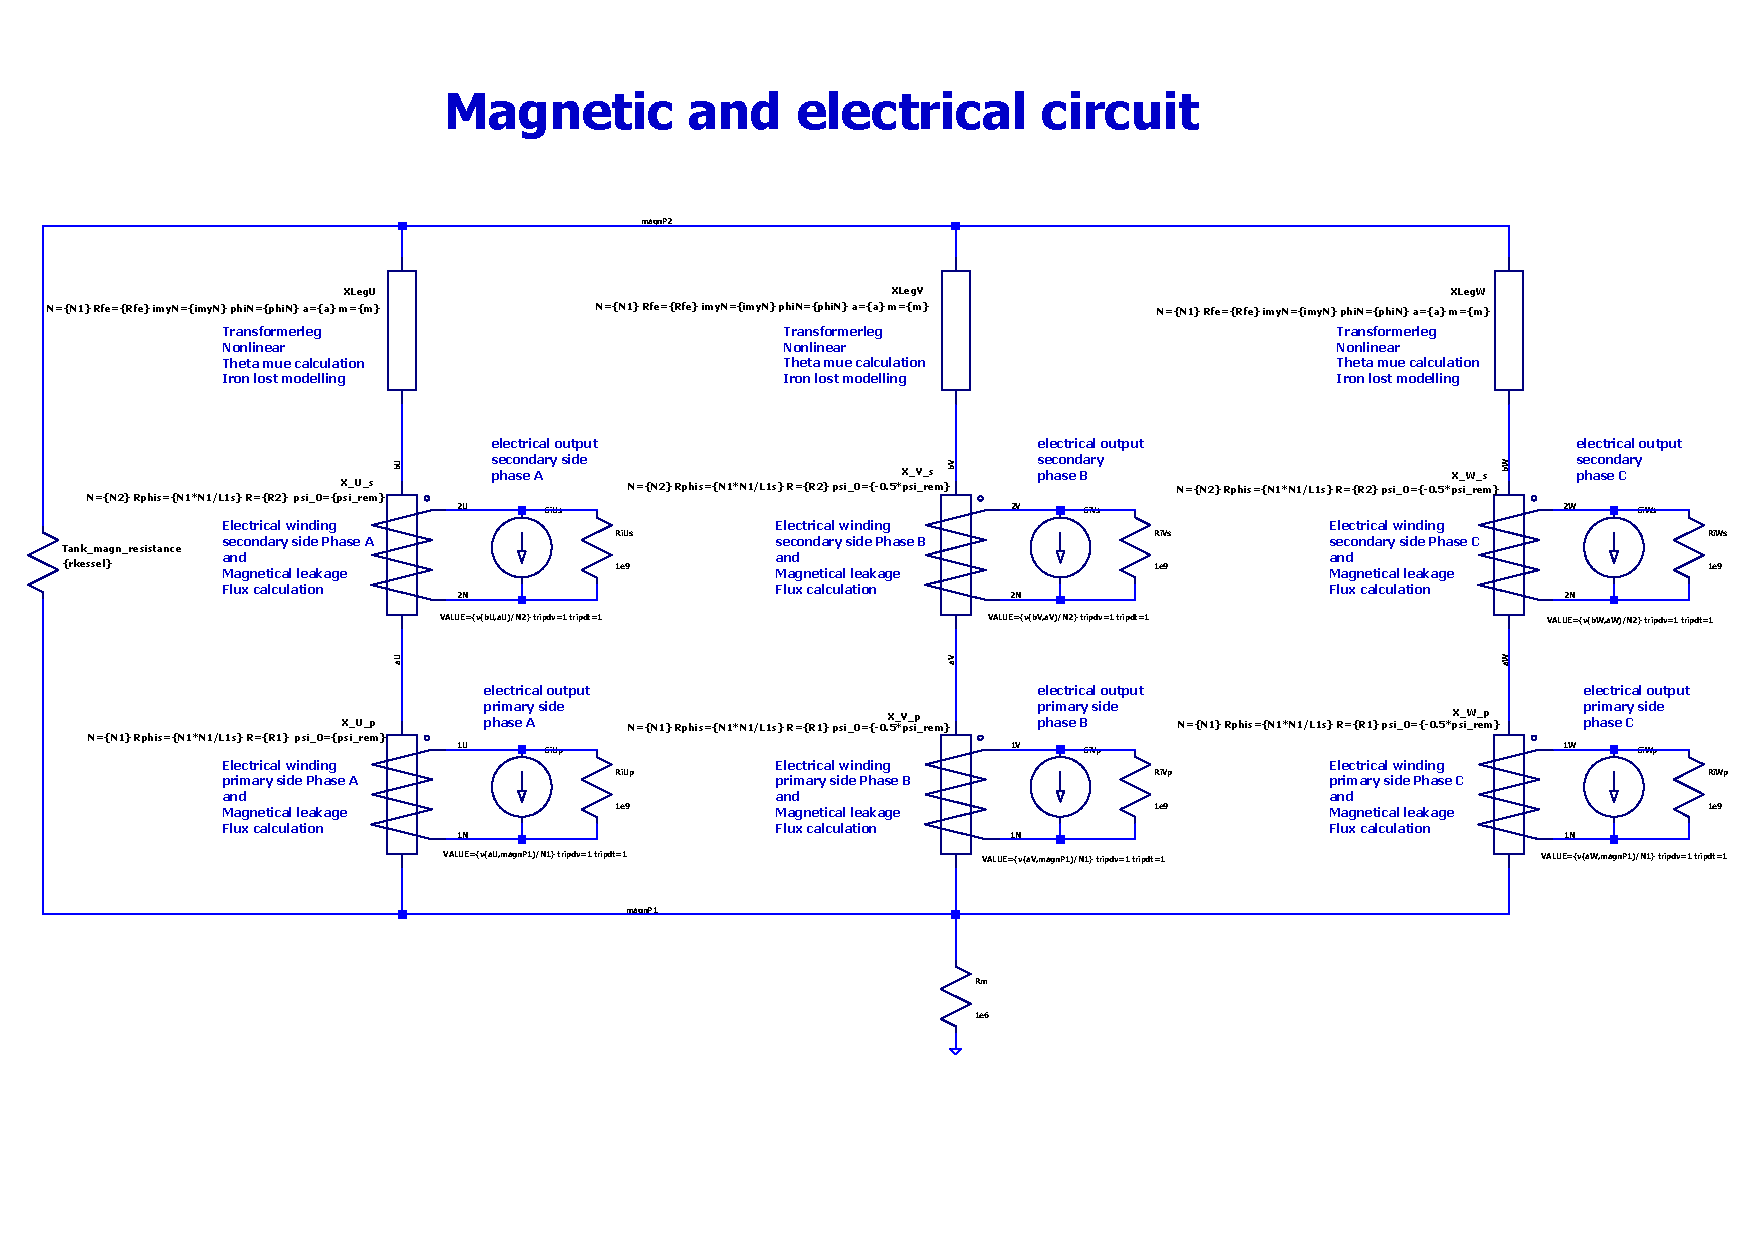
\includegraphics[width=1.5\textwidth]{figures/trafo_Yy_hierarchical_designed.pdf}
\end{widefigure}

%\begin{figure}[H]
%	\centering
%	\includegraphics[width=0.99\textwidth]{figures/Transformer_and_shunt_reactor_AC_Schematic}
%	\caption{Schematic for the Transformer and shunt reactor circuit.}
%	\label{fig:Transformer_and_shunt_reactor_AC_Schematic}
%\end{figure}


\begin{figure}[H]
	\centering
	\includegraphics[width=0.90\textwidth]{figures/winding_and_transformerleg.pdf}
	\caption{One winding and one leg of the transformer model}
	\label{fig:Transformer_and_shunt_reactor_AC_Waveform}
\end{figure}

%\begin{figure}[H]
%	\centering
%	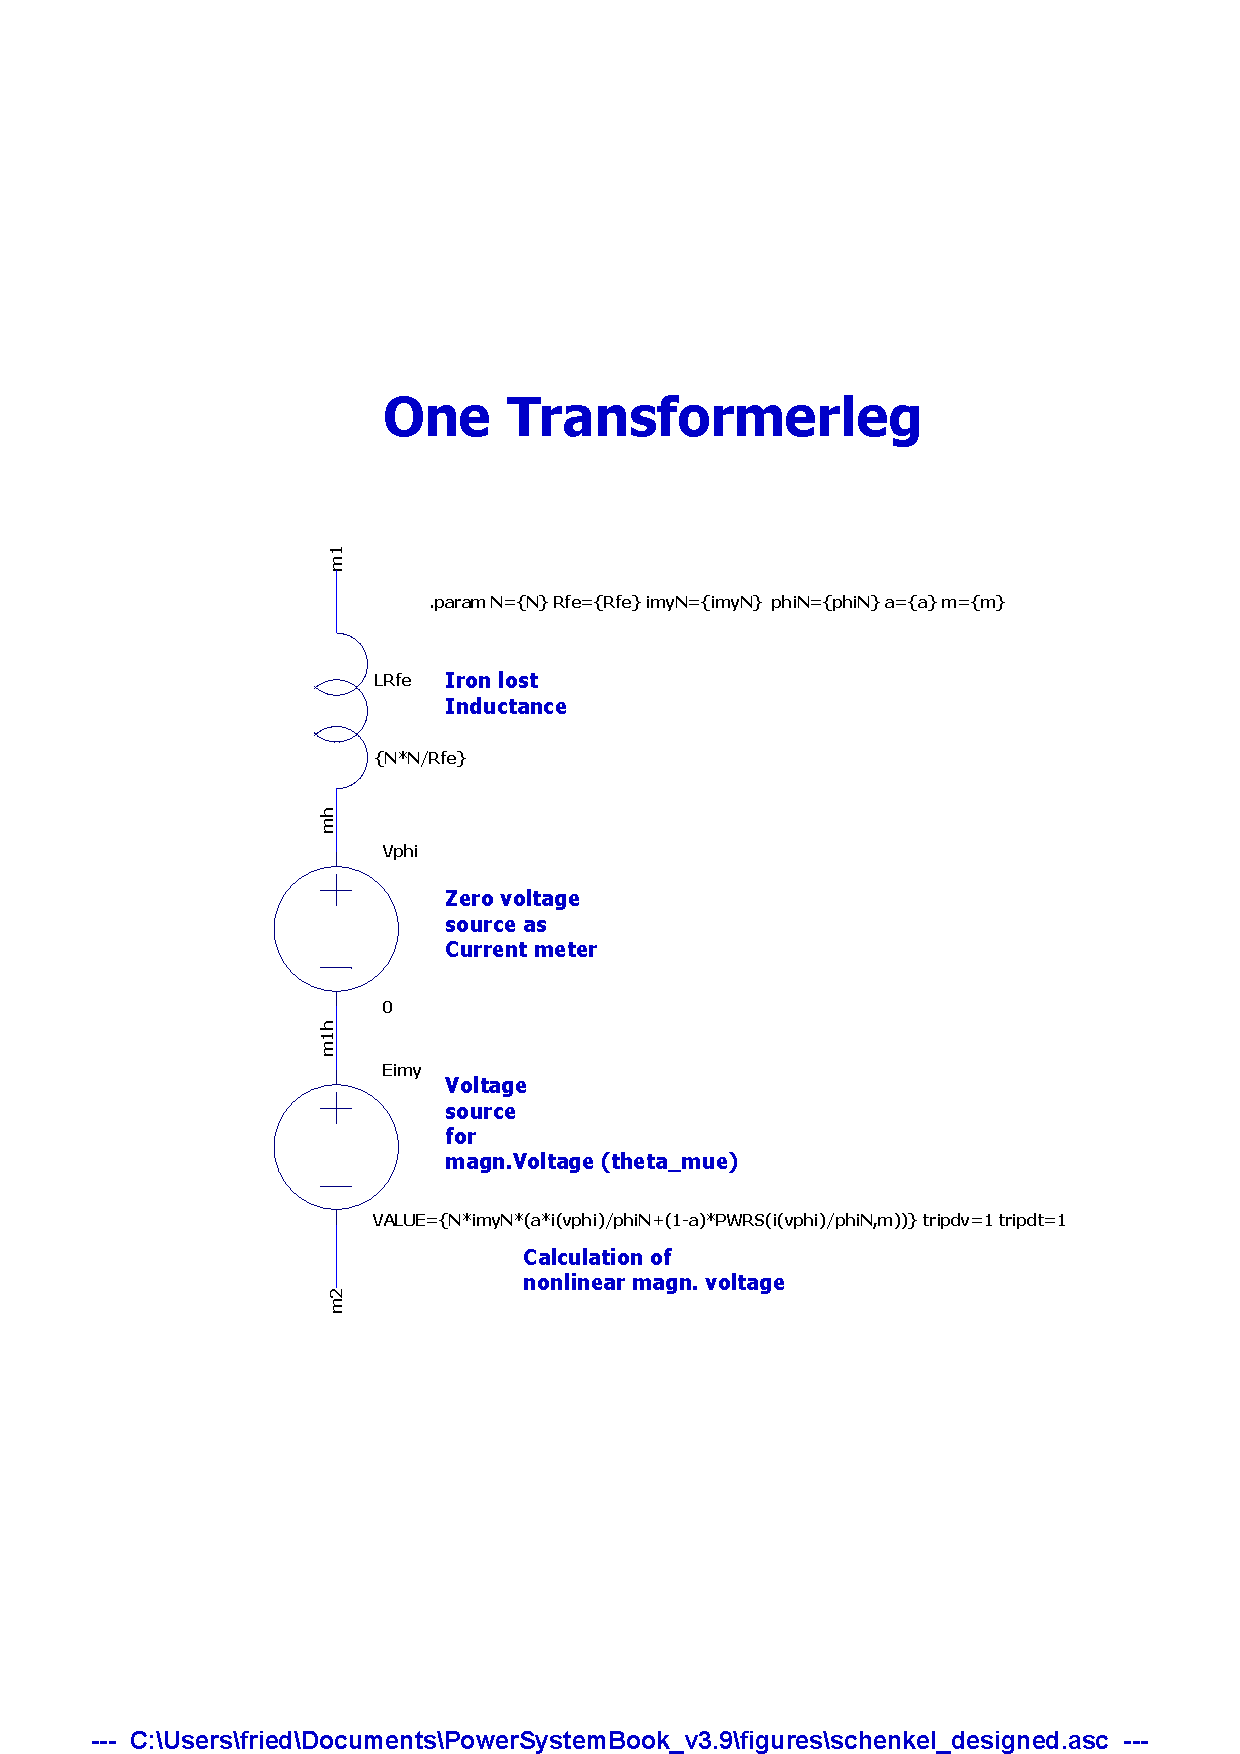
\includegraphics[width=0.90\textwidth]{figures/schenkel_designed.pdf}
%	\caption{One Leg of the transformer model}
%	\label{fig:Transformer_and_shunt_reactor_AC_Waveform}
%\end{figure}

\pagebreak

\begin{lstlisting}[style=LTspice,caption={Behavioral implementation of a three-phase transformer.},label={lst:Three phase transformer}]

1 .SUBCKT RUYy0_400k_120k_300MVA 1U 1V 1W 1N 2U 2V 2W 2N
2 + PARAMS:
3 + SN=300e6
4 + U1Nenn=400e3
5 + U20=120e3
6 + fn={fn1}
7 + N1=1000
8 + uR=0.002
9 + uX=0.2
10 + i0=0.0006
11 + p0=0.0004
12 + a=0.75 ; FS
13 + m=9;FS
14 + psi_0=0 ; Remanence-parameter 0,1,-1
15 + psir=1
16 + psis=-0.5
17 + psit=-0.5
18 + tpsi0=1000s ; Remanence-timepoint
19 + tpsid=0.1ms ; On-time of remanent flux
20 + ron=0.00001 ; On - Parameter of switcher for remanent flux
21 + bf=0 ; bf=1 -> middle leg with shorter magn. path correction factor
22 + rkessel=6e5 ; Tank resistance
23 + l_=0
24 + middle=0
25 + stproz=1.0
26 + ctrl={1+(l_-middle)*stproz/100} ; simple Tap changer
***************************************************************************
27 Xu 1U 1N 2U 2N magn1 magn2 Trafoschenkel2_Yy
28 + PARAMS:
29 + SN={SN/3} U1N={U1Nenn/sqrt(3)} U20={U20/sqrt(3)} fN={fN} N1={N1} uR={uR}
30 + uX={uX} i0={i0*IF(bf==0,1,1.2)} p0={p0*IF(bf==0,1,1.2)} a={a} m={m}
31 + psi_0={psir*psi_0} tpsi0={tpsi0} tpsid={tpsid} ron={ron} ctrl={ctrl}
***************************************************************************
32 Xv 1V1N 2V 2N magn1 magn2 Trafoschenkel2_Yy
33 + PARAMS:
34 + SN={SN/3} U1N={U1Nenn/sqrt(3)} U20={U20/sqrt(3)} fN={fN} N1={N1} uR={uR}
35 + uX={uX} i0={i0*IF(bf==0,1,0.6)} p0={p0*IF(bf==0,1,1.2)} a={a} m={m}
36 + psi_0={psir*psi_0} tpsi0={tpsi0} tpsid={tpsid} ron={ron} ctrl={ctrl}
***************************************************************************
37 Xw 1W 1N 2W 2N magn1 magn2 Trafoschenkel2_Yy
38 + PARAMS:
39 + SN={SN/3} U1N={U1Nenn/sqrt(3)} U20={U20/sqrt(3)} fN={fN} N1={N1} uR={uR}
40 + uX={uX} i0={i0*IF(bf==0,1,1.2)} p0={p0*IF(bf==0,1,1.2)} a={a} m={m}
41 + psi_0={psir*psi_0} tpsi0={tpsi0} tpsid={tpsid} ron={ron} ctrl={ctrl}
***************************************************************************
42 Rm magn1 0 1MEG
43 Rkessel magn1 magn2 {rkessel}
44 RGND1U 1U 0 1e12
45 RGND1V 1V 0 1e12
46 RGND1W 1W 0 1e12
47 RGND2U 2U 0 1e12
48 RGND2V 2V 0 1e12
49 RGND2W 2W 0 1e12
50 RGND1N 1N 0 1e12
51 RGND2N 2N 0 1e12
52 .ENDS
**************************************************************
54 .SUBCKT Trafoschenkel2_Yy 1_1 1_2 2_1 2_2 magnP1 magnP2
55 + PARAMS:
56 + SN=10kVA
57 + U1N=400V
58 + U20=400V
59 + fn={fn1}
60 + N1=1000
61 + uR=0.04
62 + uX=0.08
63 + i0=0.05
64 + p0=0.005
65 + a={0.3} ; FS
66 + m={7} ; FS
67 + psi_0=0 ; Remanenzparameter 0,1,-1
68 + tpsi0=40ms
69 + tpsid=0.1ms
70 + ron=0.00001
71 + ctrl=1
72 .PARAM
73 + I1N={SN/U1N}
74 + Z1N={U1N/I1N}
75 + omegaN={(2*pi)*fN}
76 + R1={Z1N*uR/2}
77 + L1s={Z1N*uX/2/omegaN}
78 + RFe={U1N*U1N/(p0*SN)}
79 + N2={N1*U20/U1N}
80 + R2={R1*N2/N1*N2/N1}
81 + Xh={(U1N*U1N)/(SN*sqrt(i0*i0-p0*p0))} ;FS
82 + iu={U1N/Xh} ;FS
83 + ImyN={sqrt(2)*iu} ;FS
84 + phiN={sqrt(2)*U1N/omegaN/N1}
85 + a={a} ; FS
86 + m={m} ; FS
************************************************************************
87 * Windingscurrents
88 Gi1 1_1 1_2 VALUE={v(a,magnP1)/(N1*ctrl)}
89 Rpi1 1_1 1_2 1000MEG
90 Gi2 2_1 2_2 VALUE={v(b,a)/N2}
91 Rpi2 2_1 2_2 1000MEG
92 * Windings
************************************************************************
93 X_W1 magnP1 a 1_1 1_2 winding_Yy
94 +PARAMS: R={R1} N={N1} Rphis={N1*N1/L1s}
95 +psi_0={psi_0*phiN} tpsi0={tpsi0} tpsid={tpsid} ron={ron} ctrl={ctrl}
************************************************************************
96 X_W2 a b 2_1 2_2 winding_Yy
97 +PARAMS: R={R2} N={N2} Rphis={N1*N1/L1s}
98 +psi_0={psi_0*phiN} tpsi0={tpsi0} tpsid={tpsid} ron={ron} ctrl=1
***********************************************************************
99 * Iron leg
100 X_SCH b magnP2Leg_Yy PARAMS:
101 + N={N1} RFe={RFe} ImyN={ImyN} ctrl={ctrl}
102 + phiN={phiN} a={a} m={m}
103 .ENDS
104 *******************************************************************
105 .SUBCKT winding_Yy ma mb ea eb
106 +PARAMS: R=1 N=1 Rphis=1 psi_0=0 tpsi0=1000s 
+   tpsid=0.1ms ron=0.00001 ctrl=1
107 Gphi ma mb VALUE={v(phi)}
108 Rphis ma mb {Rphis*ctrl*ctrl}
109 ; Flux phi 
110 Gp 0 phi VALUE={(v(ea,eb)-R*ctrl*v(mb,ma)/(N*ctrl))/(N*ctrl)}
111 Cp phi 0 1 IC=0
112 Rpphi 01000MEG
113 Vctrl ctrl 0 pwl 0s 0v {tpsi0+1p} 0v {tpsi0+tpsid+2p} 1V 
+   v{tpsi0+2*tpsid+3p} 1v {tpsi0+3*tpsid+4p} 0v
114 S1 phi phix ctrl 0 MS1
115 .model MS1 SW(Ron={Ron} Roff=1e9 Vt=0.9 Vh=0 Lser=0 Vser=0)
116 E1 phix 0 value={psi_0}
117 .ENDS ;
118 ******************************************************************
119 * magnetic leg
120 .SUBCKT Leg_Yy m1 m2
121 +PARAMS: N=1 RFe=1 ImyN=1 a=1 phiN=1 m=9 ctrl=1
122 LRFem1 mh {N*ctrl*N*ctrl/RFe} Rser={0.001m*N*N/RFe} ; Rser=parasitic Value
123 vphi mh mh1 0
124 rphi mh 0 1e12
125 Eimy mh1 m2
126 +VALUE={N*imyN*(a*i(vphi)/phiN+(1-a)*PWRS(i(vphi)/phiN,m))}
127 .ENDS;
128 ******************************************************************

\end{lstlisting}



%\begin{figure}[H]
%	\centering
%	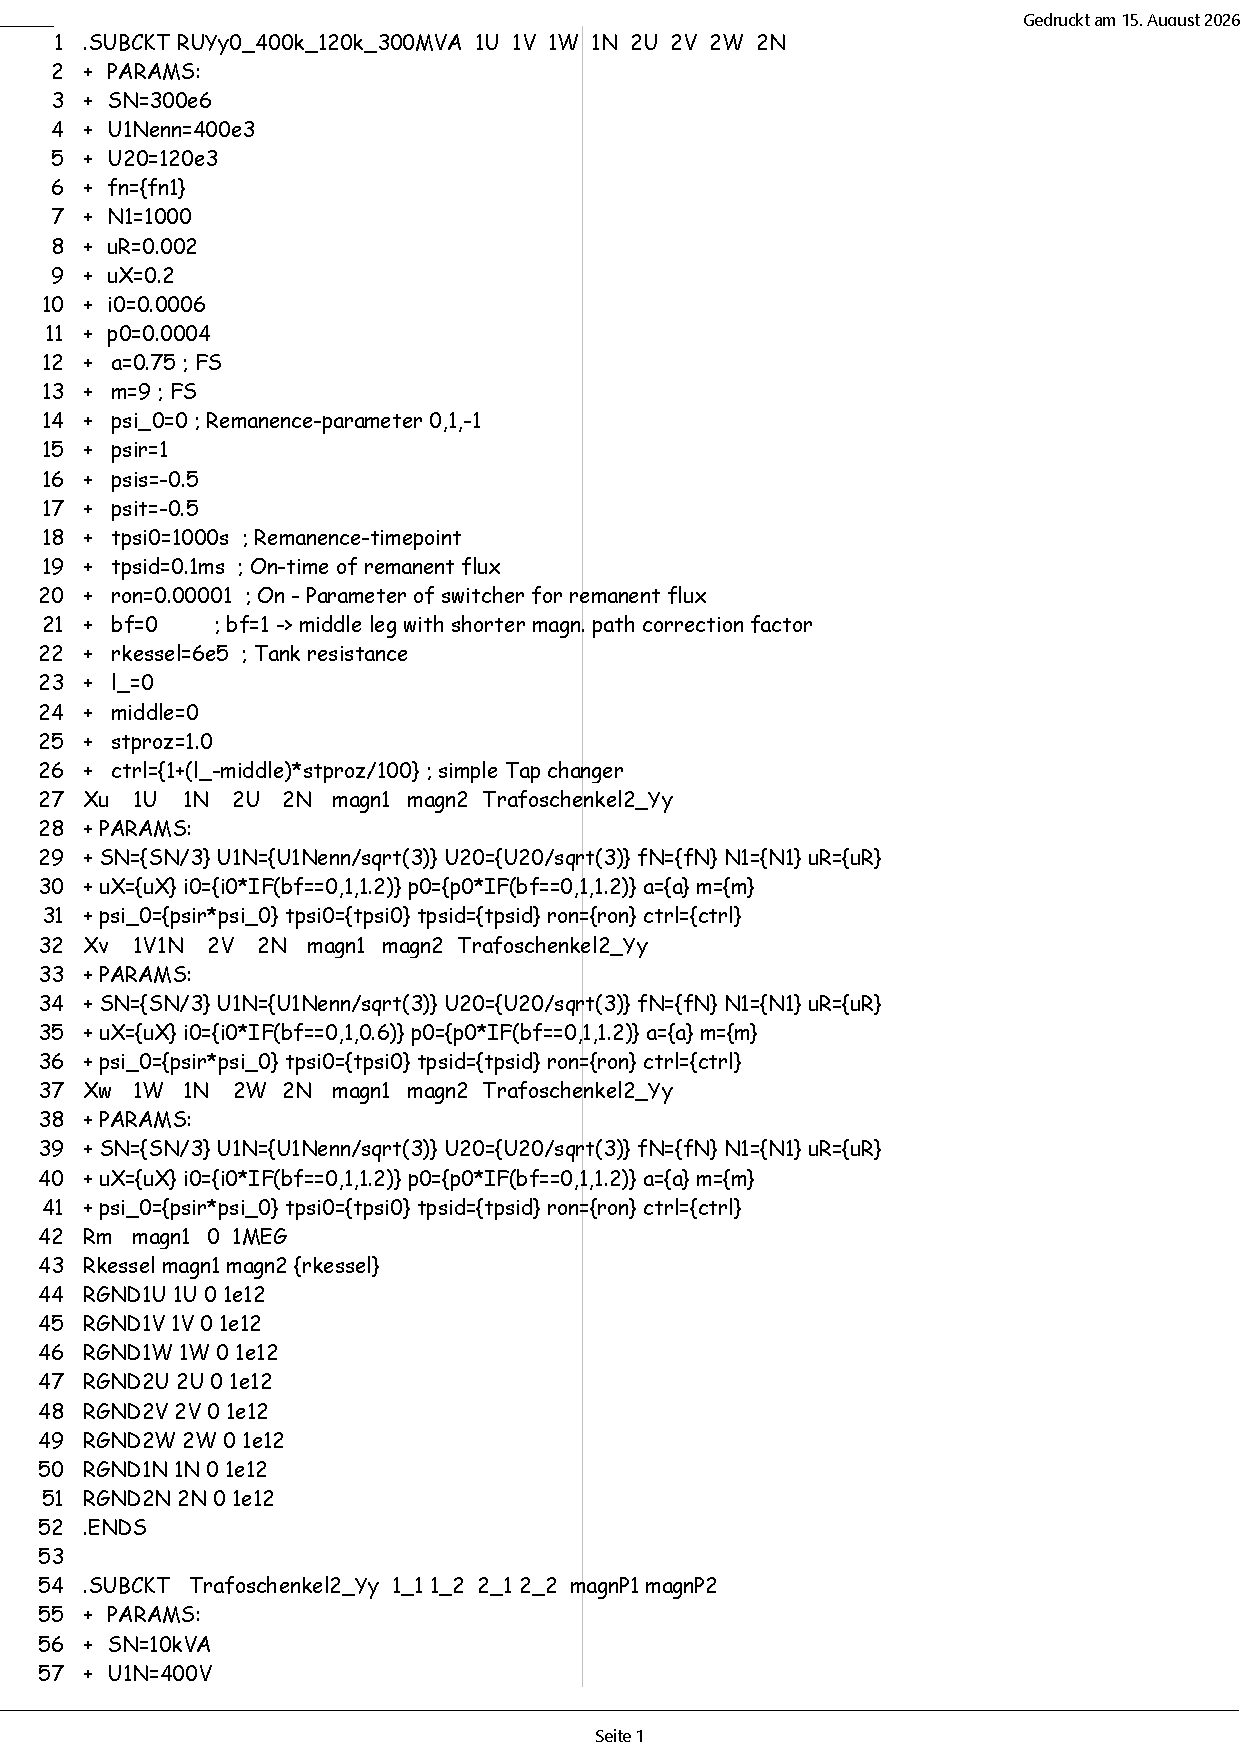
\includegraphics[width=0.90\textwidth]{figures/Transformer_SpiceCode1 1.pdf}
%	\caption{Spice code for transformer model Page1 of 3}
%	\label{fig:Transformer_and_shunt_reactor_AC_Waveform}
%\end{figure}
%
%\begin{figure}[H]
%	\centering
%	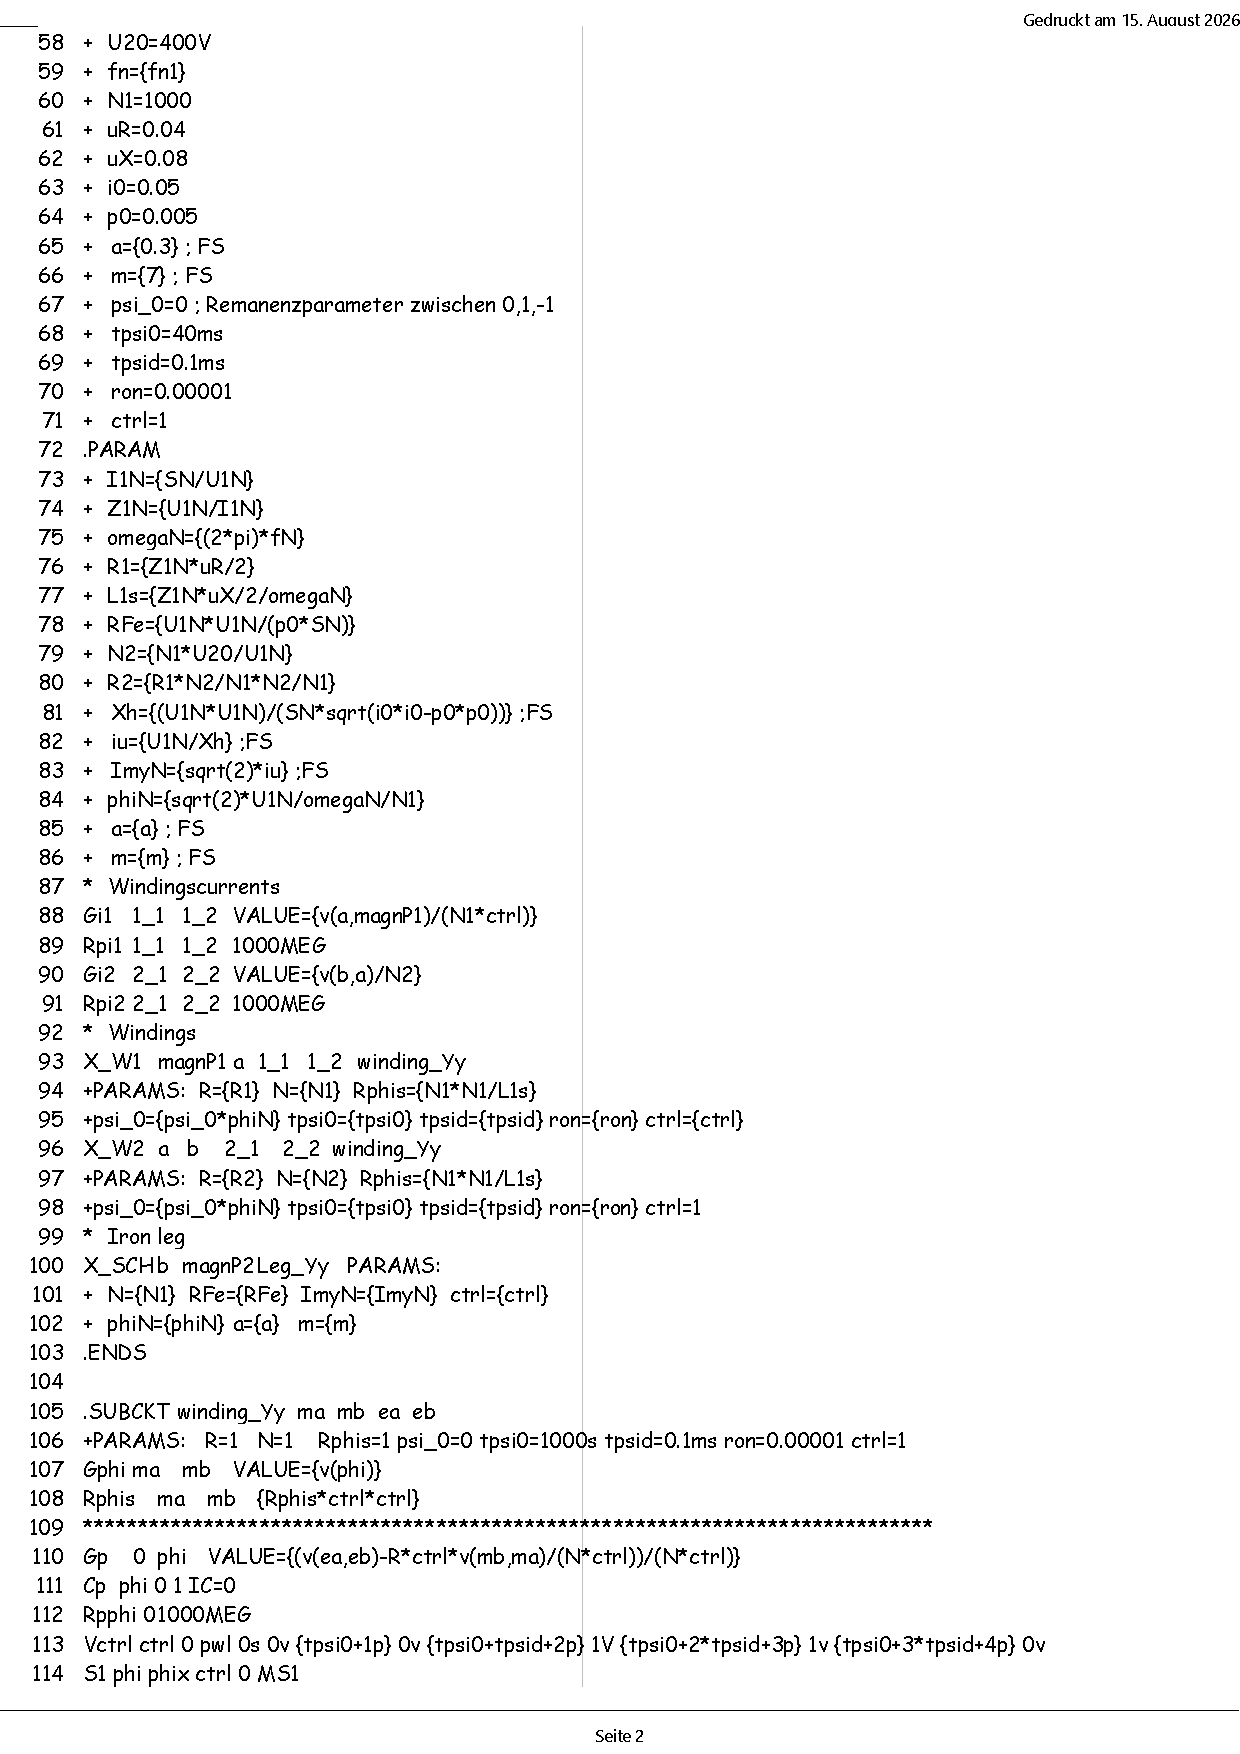
\includegraphics[width=0.90\textwidth]{figures/Transformer_SpiceCode1 2.pdf}
%	\caption{Spice code for transformer model Page2 of 3}
%	\label{fig:Transformer_and_shunt_reactor_AC_Waveform}
%\end{figure}
%
%\begin{figure}[H]
%	\centering
%	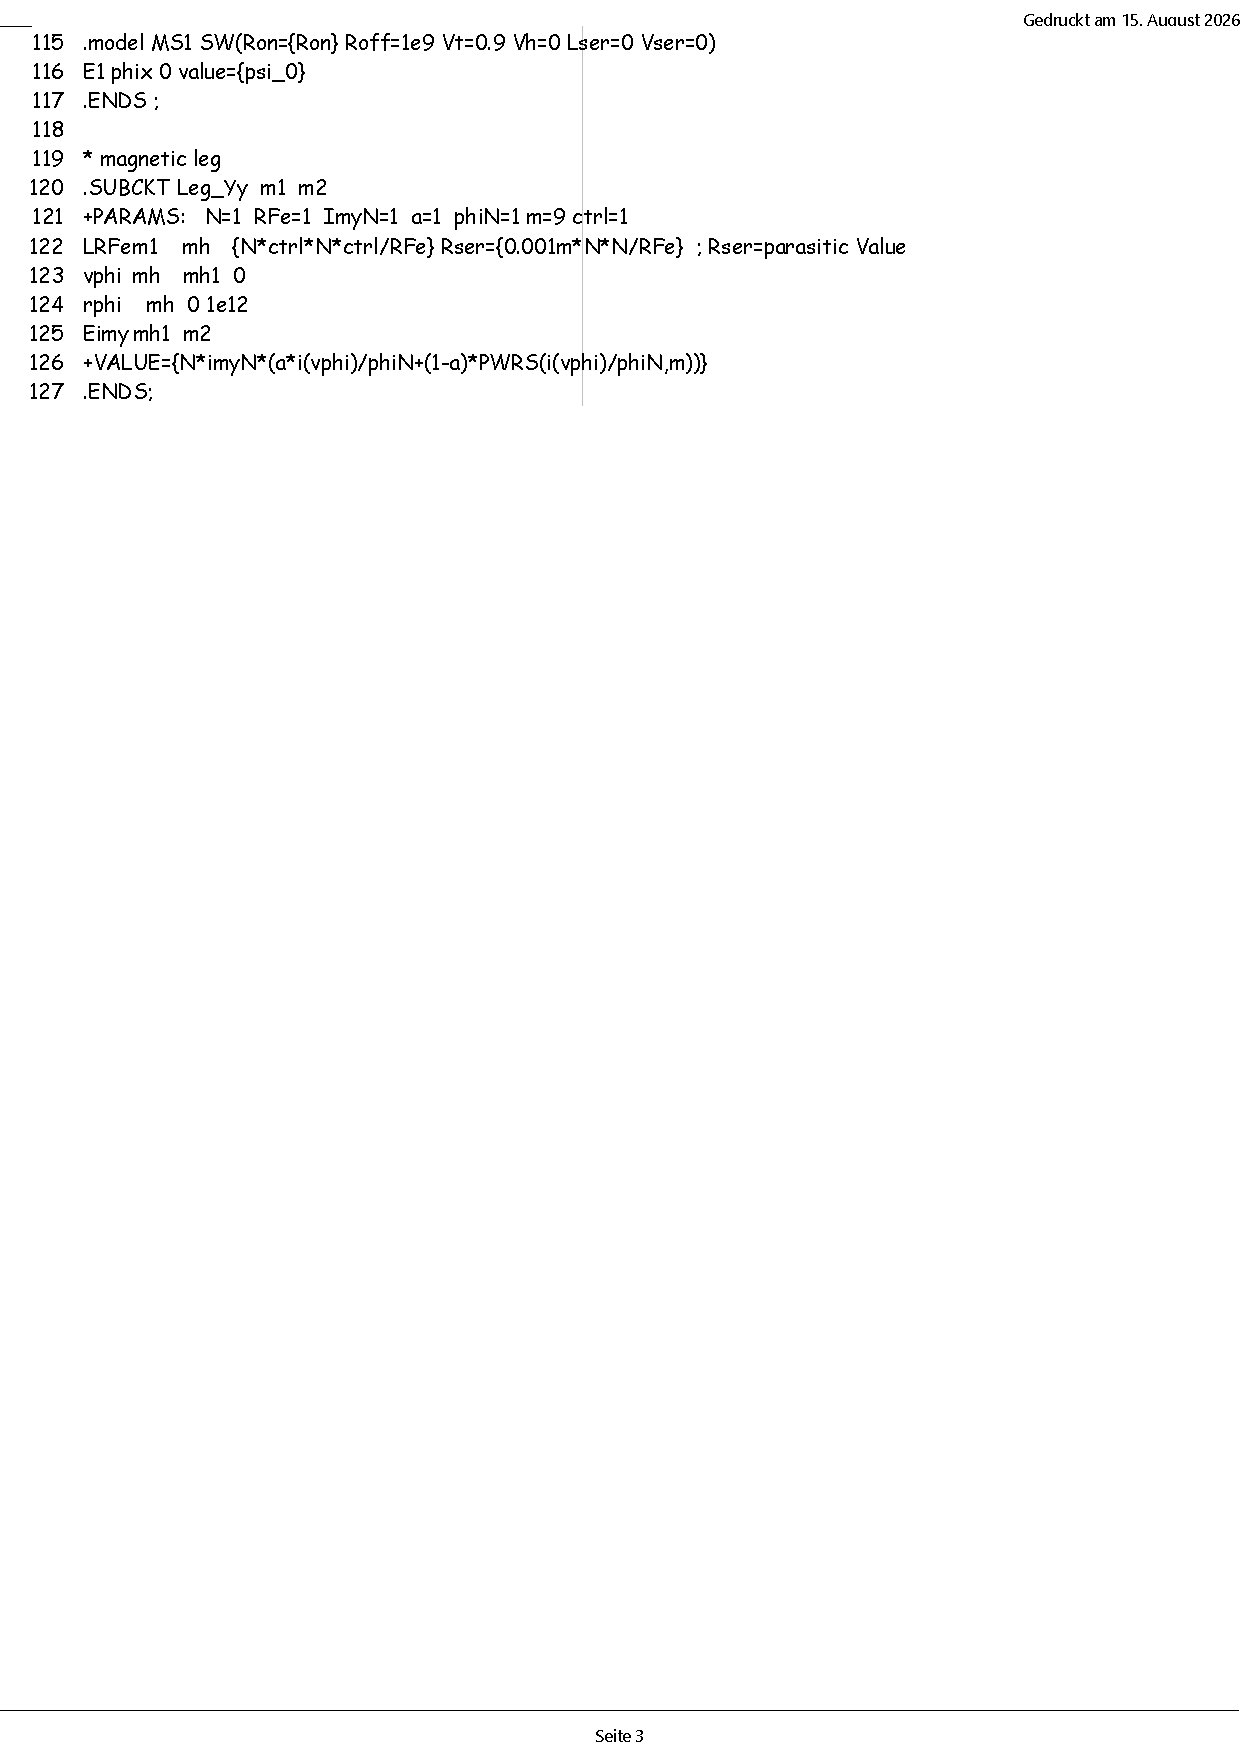
\includegraphics[width=0.90\textwidth]{figures/Transformer_SpiceCode1 3.pdf}
%	\caption{Spice code for transformer model Page3 of 3}
%	\label{fig:Transformer_and_shunt_reactor_AC_Waveform}
%\end{figure}


	
